
\chapter{Evaluation}\label{chapter:evaluation}

In this chapter, the approach presented in the previous chapter is evaluated regarding performance, safety properties, and general feasibility. For this, a number of tests were conducted which are presented in the following. But first, the experiment setup is thoroughly described.

\section{Benchmarks}

\subsection{Experimental Setup}\label{sec:testsetup}

The network topology used in the tests is depicted in \autoref{fig:network-topology}. In the local test environment ("on-premise") there was a cluster of three ARM-based SOCs\footnote{System on a Chip} (Raspberry Pi 3) whose network interfaces were connected by a Gigabit LAN switch (left-hand side). The three nodes represent on-board computing devices in a hypothetical vehicle. Connected to the LAN was also a workstation which fulfilled the sole purpose of orchestrating the tests, \ie , it was not directly involved in the test execution per se. The local test environment was connected to the remote data center over the open Internet via 100 Mbit/s connection.

\begin{figure}[htpb]
  \centering
  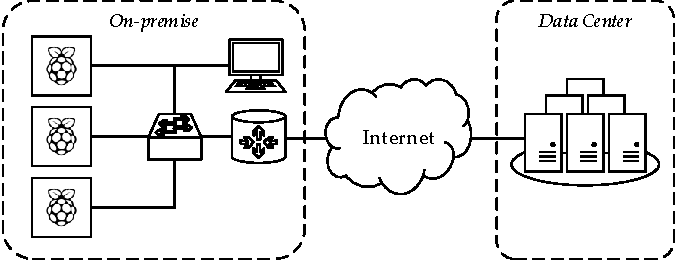
\includegraphics[width=\textwidth]{figures/network-setup}
  \caption[Network topology of the experimental setup]{The experimental setup's network topology}\label{fig:network-topology}\todo[inline]{copy rights on raspberry pi logo?}
\end{figure}
%
Representative of the "cloud" in the tests is a single root server supplied by the IaaS provider \emph{DigitalOcean}\footnote{\url{www.digitalocean.com}} (right-hand side in \autoref{fig:network-topology}). To ensure realistic latency values, a server location was chosen that was in the vicinity of the test setup -- but not too close. Considering its vicinity to Munich, Frankfurt (Main) was a suitable choice. The two cities are about 300 km away from each other (as the crow flies).

Throughout the whole study the software composition remained unchanged. As DDS implementation \emph{OpenDDS}\footnote{\url{www.opendds.org}} was chosen. The middleware was configured to utilize dynamic service discovery (no service repository) and RTPS over UDP as wire protocol. The optional Data Local Reconstruction Layer (DLRL) was used, by which messages are converted into type safe data structures. This causes some overhead which was evaluated and discussed in \autoref{sec:ddslatency}. Generally, default QoS settings were used for the tests, except in cases where a point was made to explicitly deviate from the defaults, \eg , the \liveliness\ settings in \autoref{sec:failovertest}. Moreover, all benchmarks were programmed in C++ to maximize their run time performance.

Naturally, in the benchmarks concerned with the testing of \wnet  , containers were connected by means of a \wnet\ overlay network. For the connection between all local nodes (on-premise), fast datapath forwarding mode was used. Due to the characteristics of the network between the local nodes and the cloud, fast datapath was not applicable for that connection. Consequently, local containers and cloud containers were connected via sleeve mode.

The detailed specifications of the involved computing nodes and the employed software are given in \autoref{tab:test-specs}
%
\begin{table}[htpb]
  \caption[Test environment specifications]{Test environment specifications}\label{tab:test-specs}\todo[inline]{check again}
  \centering
  \begin{tabular}{p{0.235\textwidth} | p{0.335\textwidth}  p{0.335\textwidth}}
    \toprule
       & \textbf{On-premise} & \textbf{Remote} \\
    \midrule
    	Description & Raspberry Pi 3 Model B  & DigitalOcean 1 GB Droplet\\
    	Number of nodes & 3  & 1\\
    	\midrule
    	Operating system & Raspbian GNU/Linux 9.3  & Ubuntu 16.04.3 LTS\\
    	Kernel & 4.9.59-v7+ w/ real-time patch \emph{PREEMPT\_RT} 4.4.9-rt17 & 4.4.0-112-generic \\
      CPU & ARMv7 rev 5  Quad Core (1.2 GHz) & Intel(R) Xeon(R) E5-2650 v4 Single Core (2.20GHz) x86\_64 \\
      Memory (RAM) & 1 GB & 1 GB  \\
      Network connection  & 100 Mbit/s & 40 Gbit/s\\
      \midrule
      DDS & \multicolumn{2}{c}{OpenDDS 3.12.1}\\
      Docker  & \multicolumn{2}{c}{17.11.6-ce}\\
      \wnet & \multicolumn{2}{c}{2.2.0}\\
    \bottomrule
  \end{tabular}
\end{table}
%
%
%
%
%
%
%
%
%
%

\subsection{Latency Benchmark} \label{sec:plainlatency}

\paragraph{Motivation.} An essential non-functional requirement for computer networks is responsiveness. An often-used metric for responsiveness is latency which is measured by the time it takes for a packet to be sent from one peer to another and back again. The unit of this measure is round-trip time (RTT), which is typically indicated in milliseconds. 

To evaluate the aptitude of the proposed approach it is essential to consider the latency overhead that overlay networks induce. Since the approach is intended to work over the Internet, and public networks are inherently insecure, encryption is vital. Thus, in addition to the overhead induced by the overlay network itself, the overhead caused by encryption is also of interest. Hence, tests are needed measuring latency not only of \emph{plain} overlay networks but also of \emph{encrypted} overlay networks.


\paragraph{Methodology.} 

\begin{figure}[htpb]
  \centering
  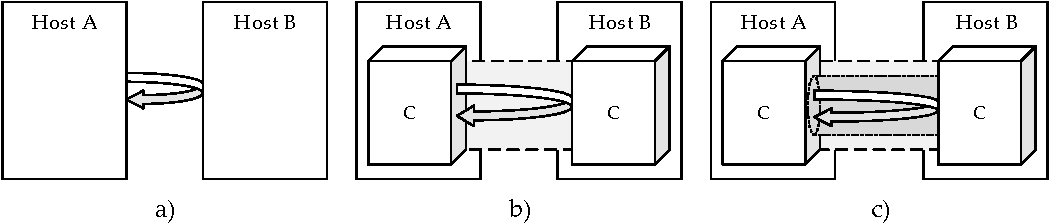
\includegraphics[width=\textwidth]{figures/ping-test}
  \caption[Latency experiment setup]{Latency experiment setup. a) \experim{Plain}: two hosts connected without overlay network. b) \experim{Weave}: two containers connected via \wnet . c) \experim{Encrypted}: two containers connected via encrypted \wnet\ .}\label{fig:latency-setup}
\end{figure}

In this test, latency was measured between two hosts connected over the Internet, both with, and without overlay-enabled container networking. A constant stream of ping messages was sent from one of the Raspberry Pis to the remote host. The tests were repeated with multiple payload sizes to factor in the influence of message size on round trip times. The Linux tool \emph{ping}, which pings hosts via ICMP Echo Requests and Replies, was employed for the measurements. 

Three experiments were conducted, comparing the average latencies of plain, host-to-host communication ("\experim{Plain}"), via \wnet\ ("\experim{Weave}") and when employing encryption over \wnet\ ("\experim{Encrypted}") (\cf \autoref{fig:latency-setup}). \experim{Plain} was used as baseline on the basis of which the two consecutive experiments were evaluated. For each experiment and message size, 300 ping messages were sent. The sending peer would wait for the response of the previous message before sending another request. Thus, only one transaction was in flight at a time.


\paragraph{Results.} 

\autoref{fig:latency-relative} depicts the absolute and relative latency measures of the tested network modes. Values represent the average round trip time of the 300 sent messages. The relative overhead is calculated from ratio of \experim{Weave} and \experim{Encrypted} when compared to \experim{Plain}, respectively. The results show that the network latency induced by \wnet\ (without encryption) is hardly measurable and therefore negligible. Message size has no influence whatsoever in this comparison. 


\begin{figure}[htpb]
  \centering
  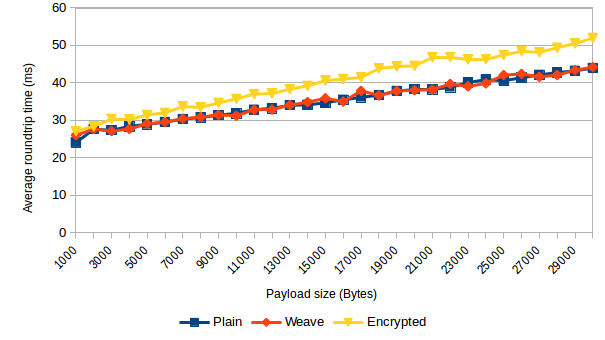
\includegraphics[width=0.49\textwidth]{figures/latency-absolute}
  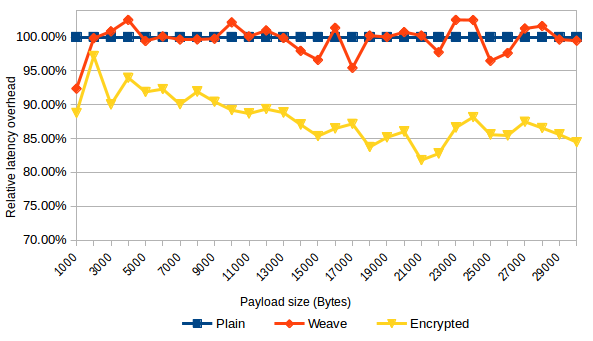
\includegraphics[width=0.49\textwidth]{figures/latency-relative}
  \caption[Latency overhead]{Absolute (a) and relative (b) latency overhead of \experim{Weave} and \experim{Encrypted} over \experim{Plain}}\label{fig:latency-relative}
\end{figure}

However, the tests revealed that encryption over \wnet\ (\experim{Encrypted}) adds quite a hefty base overhead which further increases with message size. For the smallest messages the overhead started at roughly 5\% and went up to over 15\% for messages with 30 KB payload. The encryption overhead may therefore be considered significant.

\begin{figure}[htpb]
  \centering
  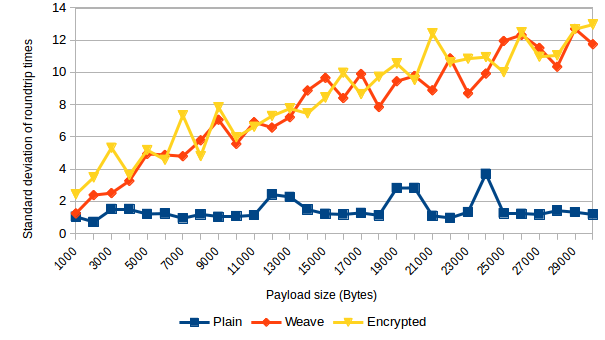
\includegraphics[width=0.8\textwidth]{figures/latency-stdev}
  \caption[Latency deviation]{Standard deviation of latencies in the scenarios \experim{Plain}, \experim{Weave} and \experim{Encrypted}}\label{fig:latency-stdev}
\end{figure}

Another insight worth mentioning is that \wnet\ added significant deviations in latency that increased with message size (\cf \autoref{fig:latency-stdev}). Whether the connection was encrypted or not made little difference. Real-time systems need to behave in a predictable manner. The experiments show that routing traffic through overlay networks had a substantial, negative impact on predictability of the communication channel. From the viewpoint of real-time systems this is a serious drawback of the presented approach. 



%
%
%
%
%
%
%
%
%
%

\subsection{Throughput Benchmark} \label{sec:throughput}

\paragraph{Motivation.} Another important metric for network performance is throughput. Throughput is a measure for how much data can be transmitted per time. Since little data is available on \wnet 's throughput performance, according tests were conducted.

\paragraph{Methodology.} To measure throughput, the tool \emph{iperf3}\footnote{\url{www.iperf.fr}} was used. iperf continuously sends data from one node to another over a TCP/IP connection. From the volume of the transmitted data and the duration of the transmission, network throughput can be deduced. iperf was set to transmit data for a relatively long time period of 30 seconds to produce meaningful results. As in the previous test, three scenarios were tested:  \experim{Plain}, \experim{Weave}, and \experim{Encryped}. Explanations of these scenarios can be taken from the previous test.

\paragraph{Results.} The results of this benchmark are depicted in \autoref{fig:throughput}. The results show that unencrypted \wnet\ adds a minor throughput overhead when compared to \experim{Plain} scenario (5\%). When adding encryption to the overlay network, a minor additional overhead can be observed. Overall, encryption incurs an overhead of 6.7\% compared to \experim{Plain}. These values can be considered decent. 


\begin{figure}[htpb]
  \centering
  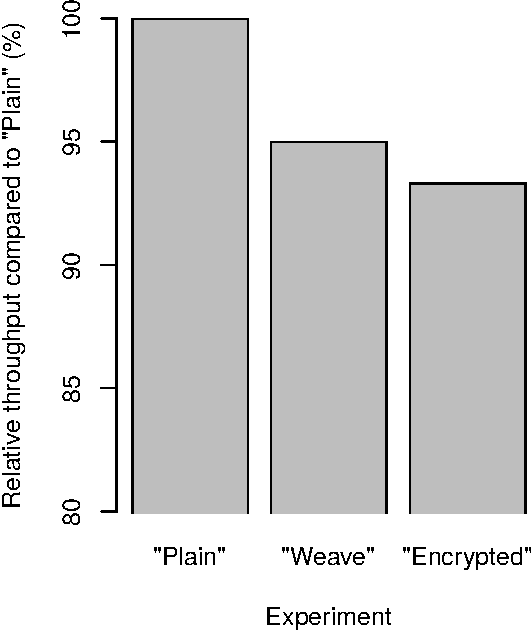
\includegraphics[width=0.8\textwidth]{figures/throughput}
  \caption[Weave throughput benchmark results]{Relative throughput in the scenarios \experim{Plain}, \experim{Weave} and \experim{Encrypted}}\label{fig:throughput}
\end{figure}


%
%
%
%
%
%
%
%
%
%

\subsection{DDS Latency Benchmark} \label{sec:ddslatency}

\paragraph{Motivation.} In the test described in \autoref{sec:plainlatency}, plain network latency was measured in different overlay network scenarios. Latencies were measured using ICMP ping so the tests did not consider the network performance of DDS. There is no data yet on how well DDS performs in SDN-based overlay networks spanning over the Internet. Hence, tests were conducted to evaluate DDS latency in such scenarios.

\paragraph{Methodology.} The methodology of this test is similar to the previous latency test in that the RTT between two hosts connected over the Internet were used as measure of latency. The ICMP ping results from that test were used as a baseline to which DDS was compared to. In order to measure DDS latency, a ping application was developed that functions similar to classic ping: a number of messages is sent from one endpoint to another, the same messages are then sent back to the sender, and finally, the current timestamp is subtracted from the returned message's timestamp to calculate the RTT. Between the reception of a returned message and the dispatch of the next message, the sender would wait for a few milliseconds to make sure that only a single message was in circulation at any time.

Of course, sending data via DDS entails a lot more than simple ICMP pings, like \eg\ the marshaling and parsing of messages. The comparison with ICMP is therefore a very ambitious one. As ICMP pings require very little processing, the largest part of the measured round trip time accounts for pure message transmission. ICMP ping is therefore a good reference point to measure the overhead induced by DDS, and in particular, RTPS. 

Again, multiple test runs with different message sizes were carried out to factor in the influence of packet fragmentation and other distorting factors. Payload sizes typical for real life applications were chosen, ranging from 100 bytes to one kilobyte. The tests in both cases (ICMP an DDS) were performed in an encrypted \wnet\ overlay network to ensure the practical relevance of the benchmark. The results presented below are the average values calculated from 300 pings per test case.


\paragraph{Results.} 
The results of the tests are presented in \autoref{fig:dds-latency}. With the experiment it was shown that DDS adds reasonable overhead when compared to the plain transmission time of ICMP ping. The overhead ranged between 11.45\% at min, and 17.55\% at max. On average, the overhead was at 14.74\%. The overhead can be explained by the fact that DDS does a lot more than just transmit data. Most notably, the enforcement of certain QoS policies took their toll on latency, as well as the marshaling, serialization and parsing of message payloads by the DLRL.


\begin{figure}[htpb]
  \centering
  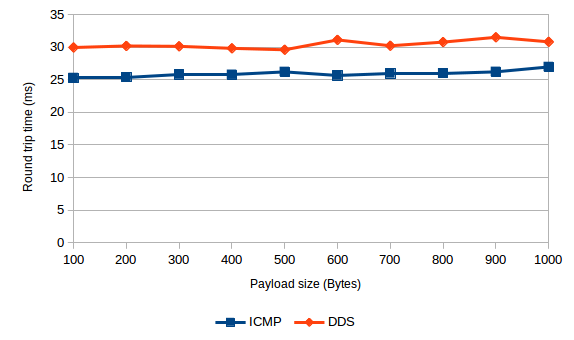
\includegraphics[width=0.7\textwidth]{figures/dds-latency}
  \caption[DDS latency benchmark results]{The average RTT of differently sized packets when using DDS versus ICMP}\label{fig:dds-latency}
\end{figure}

%
%
%
%
%
%
%
%
%
%


\subsection{Failover Test}\label{sec:failovertest}

\paragraph{Motivation.} The presented approach facilitates a wide range of innovative opportunities. For instance, consider the following scenario: A service running on an on-board computer within a vehicle suddenly fails, \eg\ due to a hardware defect. As a reaction, a fallback service needs to take over. Consider now that the fallback service is not running on another on-board computer but within the cloud. Enabled by DDS' failover qualities, the approach allows for a quick switch to the remote backup service. An interesting question is how long the whole failover process, \ie\ switching to a backup service in case of failure, takes in a cloud scenario.


\newcommand{\proda}{\texttt{S\textsubscript{main}}}
\newcommand{\prodb}{\texttt{S\textsubscript{backup}}}
\newcommand{\cons}{\texttt{S\textsubscript{consume}}}

\paragraph{Methodology.}\todo{reference failover mechanism described in previous chapter} To test the performance of DDS's failover qualities an experiment was designed to replicate a scenario in which a service fails so that another, remote service must take over operation. There are three services: two services which continuously produce data (\proda , \prodb) and one which consumes the data (\cons). \proda\ has precedence over \prodb\ (\ie\ it possesses a higher \ownership\ value) and is therefore the "main supplier", while \prodb\ is considered the "backup supplier". 

In the process of sending data, a failure of \proda\ is simulated by abruptly shutting down the application process. Once that happens, a procedure in \cons\ is triggered to determine the time span between the reception of the last message sent by \proda\ and the first message by \prodb . The resulting time is the effective gap between the reception of two messages: the last one from \proda\ and the first one from \prodb . In particular, the measured time includes
\begin{itemize}
  \item the time DDS needs to detect \proda 's change of liveliness and to propagate the change in the system
  \item the time it takes \prodb\ to take over
  \item the transmission time of \prodb 's first message to \cons
\end{itemize} 

\proda\ and \cons\ are deployed as individual applications on two of the Raspberry Pis. \prodb\ is deployed on the remote host. All communication goes through an encrypted Weave network spanning over the LAN and the cloud.

\todo[inline]{which QoS settings were used? how many test runs were conducted? Describe how clocks are synchronized between the two producing services}


\paragraph{Results.} Reliability can be ensured, even when offloading work into a remote data center.

%
%
%
%
%
%
%
%
%
%

\section{Case Study}

\paragraph{Motivation.} Motivation

%
%
%
%
%
%
%
%
%
%


\section{Limitations}

The benchmarks in the previous sections demonstrated that the approach to cloud connectivity presented in this thesis is fully functional. However, there are some limitation that need to be addressed.

Firstly, \wnet\ is not designed to be used in safety critical systems. On their website, Weaveworks make no statement about any certification efforts that make the software suitable for the use in safety-critical systems. Thus, for the time being, the given approach may only find applicability for non-safety critical functions, \eg in the context infotainment systems. However, it may be added that \wnet\ is Open Source, and as such, all underlying technologies and concepts are disclosed. Thus, it is entirely plausible to implement a thoroughly verified and tested derivative of \wnet\ tailored to safety-critical systems.

(In the context of vehicles, safety is inherently connected to the software system's security. Hence, proper methods are required to ensure the system's authenticity, confidentiality, integrity and privacy properties. The presented approach was not tested regarding these attributes. A rigor security analysis is needed to be able to make a well-founded statement about its aptitude.)

Problem with \wnet 's encryption: password-based shared secret. How to distribute shared secret? How to renegotiate shared secret? etc.


How fast can \wnet\ reconnect?

Can weave be used in PaaS systems or EC2? probably not.

It may also be noted that the Docker images presented in this thesis are by no means production ready. Although there was an effort to minimize the size of the images, in real scenarios, images would be shaved down to the bare minimum, both in terms of size and capabilities. Utilities such as compilers, build tools and generally everything which is not a prerequisite to execute a given service would be removed. The images used in this thesis serve the purpose of demonstration and thus, such measures were not taken to ensure a rapid progression of this work. More time would be needed to optimize the images for production use.


%
%
%
%
%
%
%
%
%
%
%
%
%
%
%
%
%
%
%
%
%
%
%
%
%
%
%
%
%
%
%
%